\author{Thijs Heus}
\lecture[Structure]{Structure of the code}{structure}
\section{Main files and modules}
\begin{frame}[allowframebreaks]{Files and Modules}
\mylineno=0\begin{longtable}{p{0.2\linewidth}p{0.7\linewidth}}
 LES &  Main program which calls a timing
routine and the driver, as well as the driver subroutine and the
subroutine which defines and reads the model NAMELIST file. 
\tblnewline advf &  Calculates the tendencies associated with scalar advection.
\tblnewline advl &  Calculates the tendencies associated with momentum advection.
\tblnewline defs &  Defines physical constants.
\tblnewline forc &  Case specific forcings (radiation, subsidence, \emph{etc.}).
\end{longtable}
\pagebreak
\mylineno=0\begin{longtable}{p{0.2\linewidth}p{0.7\linewidth}}
 grid &  Definition of grid, allocation of memory and I/O management
\tblnewline init &  Routines for processing input (either from
a file or the NAMELIST), definition of basic state, initialization of
fields, and definition of initial random perturbations.
\tblnewline lsvar &  computes sst, div and winds for astex case (only when lsvar=true in NAMELIST)
\tblnewline ncio &  Defines structure of ncdf output files.
\tblnewline icemcrp &  Bulk microphysical routines.
\tblnewline mpi\_interface & Definition of MPI parameters and MPI
routines for the domain decomposition (only when using MPI mode else seq\_interface).
\tblnewline prss &  Poisson solver, calculates the velocity tendencies
associated with pressure gradients, also implements time-filter for
Runge Kutta scheme and updates velocity.
\end{longtable}
\pagebreak
\mylineno=0\begin{longtable}{p{0.2\linewidth}p{0.7\linewidth}}
rad\_cldwtr & Calculates radiation properties from cloud water and effective radius.
\tblnewline rad\_corkds & Reads gas concentrations and calculates radiative properties such as optical depth and absorption coefficients.
\tblnewline rad\_d4strm & Computes radiative fluxes and optical properties for Rayleigh scattering.
\tblnewline rad\_driver & Includes background soundings for atmospheric gases.
\tblnewline rad\_gcss & Simple radiative parametrization for SW and LW fluxes (Delta-Eddigton approximation).
\tblnewline rad\_rndnmb & Contains a random number generator.
\tblnewline rad\_solver & Radiation solver.
\end{longtable}
\pagebreak
\mylineno=0\begin{longtable}{p{0.2\linewidth}p{0.7\linewidth}}
sgsm &  Subgrid scale solver.
\tblnewline srfc &  Surface boundary condition routines.
\tblnewline stat &  Routines for calculating, accumulating and outputting model
statistics.  Statistical output is provided through the course of a
simulation and tends to be problem specific.
\tblnewline step &  Time stepper.  Also includes several routines for computing
tendencies due to physical processes (Coriolis force, buoyancy) or
boundary conditions (Rayleigh friction for sponge layer near lid).
Updating of scalars is done here. CFL computations and
timestep-regridding are also here.
\end{longtable}
\pagebreak
\mylineno=0\begin{longtable}{p{0.2\linewidth}p{0.7\linewidth}}
 thrm & Thermodynamic routines for calculating
quantities like temperature, and cloud water, given the thermodynamic
state of the model, i.e., $\theta_l,q_t,\rho_0,\pi_0,\Theta_0.$
\tblnewline util & A collection of basic utilities including
boundary conditions, FFT calls, explicit array operations such as
domain or slab averaging or covariances, the tri-diagonal solver, and
some NetCDF utilities.  Many of the routines in this module make
active MPI calls.
\end{longtable}
\end{frame}
  
\section{Main variables}
\begin{frame}[allowframebreaks]{Main Variables}
\mylineno=0\begin{longtable}{p{0.25\linewidth}p{0.05\linewidth}p{0.6\linewidth}}
% Array    & Dimensionality & Field \tblnewline \hline \endhead
a\_xp,a\_xt1,a\_xt2 & 4D    & Data arrays used to summarize variables\tblnewline
a\_up,a\_vp,a\_wp & 3D    & $u^n, \; v^n, \;w^n$ \tblnewline
a\_ut,a\_vt,a\_wt & ''    & $\partial_t u, \; \partial_t v, 
\; \partial_t u$ \tblnewline  
a\_tp,a\_tt  & ''         & Liquid water potential temperature,
$\theta_l^{'\, n}, \;  \partial_t \theta_l$ \tblnewline 
a\_rp,a\_rt  & ''         & Total water mixing ratio $r_t^n, \;
\partial_t r_t$ \tblnewline 
a\_rpp,a\_rpt  & ''       & Rain mass mixing ratio $r_r^n, \;
\partial_t r_r$   (for level 3)\tblnewline  
a\_npp,a\_npt  & ''       & Rain number mixing ratio, $n_r^n, \;
\partial_t n_r$ (for level 3) \tblnewline  
a\_theta & '' & Potential temperature, $\theta$ (diagnosed from model state)\tblnewline  
rc,rv  & ''         & Condensate and vapor mixing ratio $r_c, \;
r_v$ (note that $r_c$ can be either the cloud or total condensate
mixing ratio depending on when it is accessed) \tblnewline 
press, a\_pexnr & ''   & Pressure and Exner function ($p, \pi$ respectively)  \tblnewline  
a\_scr1, a\_scr2 & '' & Three dimensional scratch arrays \tblnewline
a\_ustar, a\_tstar, a\_rstar & 2D & Surface scales, $u_*, \;
\theta_*, \; r_*$ respectively \tblnewline 
uw\_sfc, vw\_sfc, ww\_sfc & '' & Surface momentum fluxes,
$\overline{u'w'}, \;\overline{v'w'}, \;\overline{w'w'} $
respectively. \tblnewline  
wt\_sfc, wq\_sfc & '' & Surface thermodynamic fluxes,
$\overline{w'\theta'}, \;\overline{w'r'} $
respectively. \tblnewline
precip & '' &  Precipitation flux \tblnewline
dn0    & 1D &  Basic state density, $\rho_0(z).$ \tblnewline
xt, yt, zt & '' & Position of thermodynamic points \tblnewline
xm, ym, zm & '' & position of momentum points \tblnewline
dzi\_t        & '' & $1/(z_m(k) - z_m(k-1)$ \tblnewline
dzi\_m        & '' & $1/(z_t(k+1) - z_t(k)$ \tblnewline
% \hline \hline	
\end{longtable}
\end{frame}

\section{Grid and Parallelization}
\begin{frame}{The Horizontal Grid}
\begin{columns}
\begin{column}{0.5\textwidth} 

% \includegraphics<1>[height=0.7\textheight]{horgrid1.pdf}
% \includegraphics<2-3>[height=0.7\textheight]{horgrid2.pdf}
\includegraphics<4->[height=0.7\textheight]{horgrid3.pdf}
\end{column}
\begin{column}{0.45\textwidth}
 \begin{itemize}
  \item<1-> The grid is equidistant in the 2 horizontal directions
  \item<2-> 1 processor covers a certain part of the grid
  \item<3-> And has 2 ghost cells around it on all sides
  \item<4-> All processors together show a big amount of overlap
  \item<5-> Parallelization remains efficient with $>16 \times 16$ points per processor
 \end{itemize}

\end{column}

\end{columns}
\end{frame}
\begin{frame}{The Vertical Grid}
\begin{columns}
\begin{column}{0.5\textwidth} 
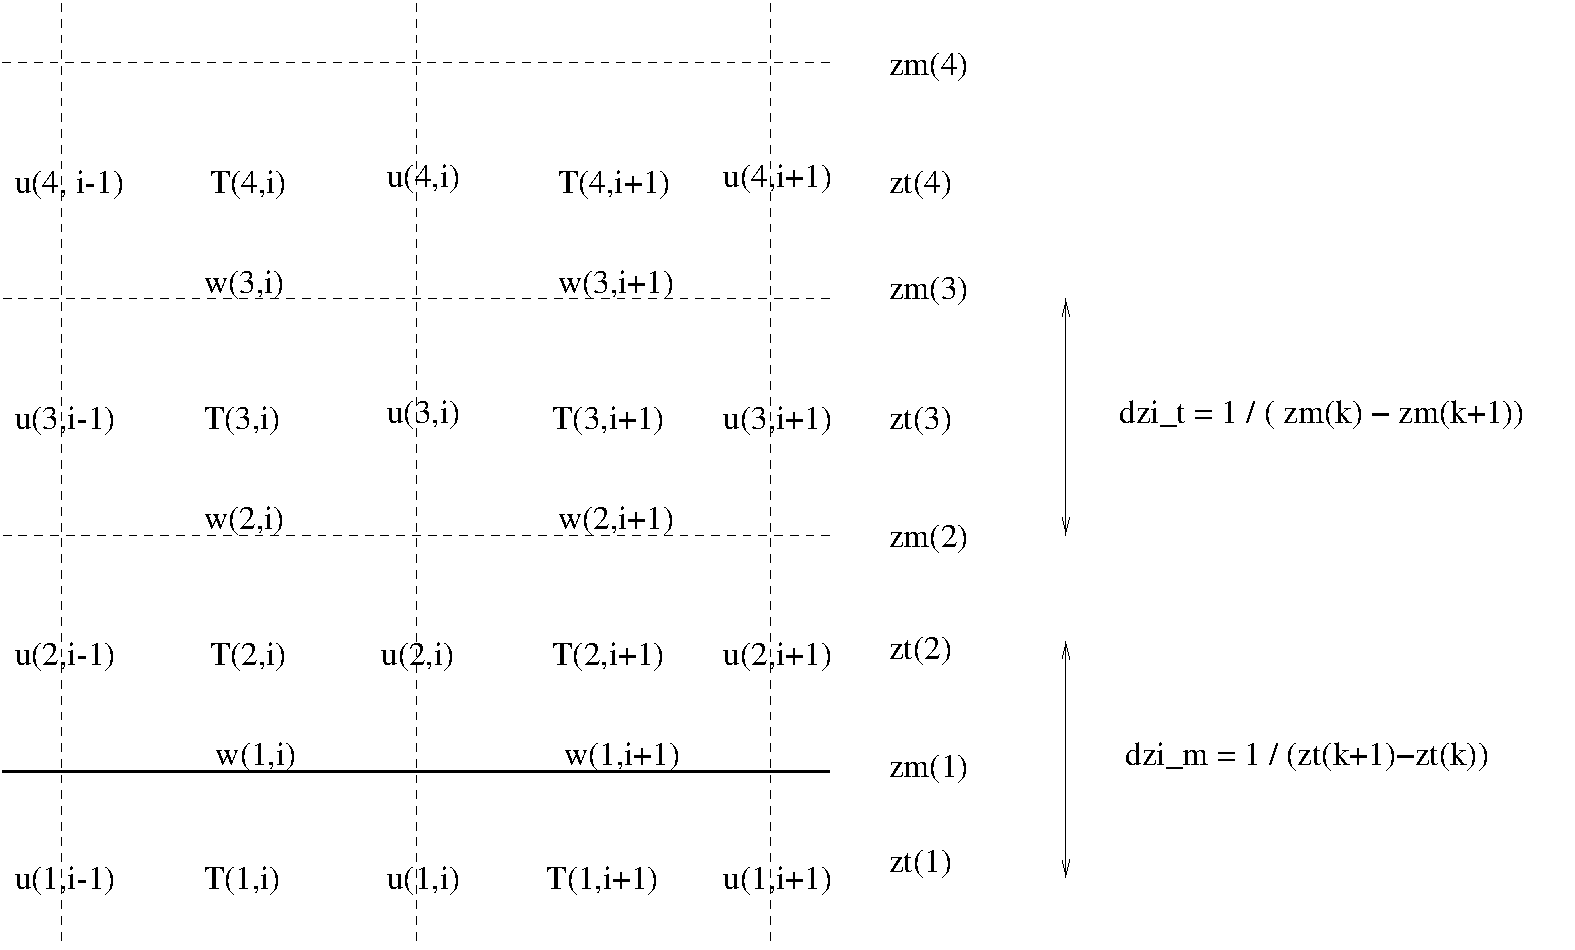
\includegraphics[height=0.5\textheight]{grid2.pdf}
\end{column}
\begin{column}{0.45\textwidth}
 \begin{itemize}
  \item The grid is staggered as a Arakawa C-grid
  \item Pressure and scalars are defined at cell center
  \item The velocities are defined at the cell faces to avoid decoupling between pressure and velocity
  \item The upper/right cell face has the same index as the cell center
 \end{itemize}

\end{column}

\end{columns}
\end{frame}
